\documentclass[14pt]{extarticle}

% Esto es para poder escribir acentos directamente:
\usepackage[utf8]{inputenc}
% Esto es para que el LaTeX sepa que el texto est en espaol:
\usepackage[spanish, activeacute]{babel}

% Paquetes de la AMS:
\usepackage{amsmath, amsthm, amsfonts}

\usepackage{extsizes}

\usepackage{pdflscape}
\usepackage{fontawesome}

\usepackage{graphicx}
\graphicspath{ {./images/} }

\usepackage[margin=1in]{geometry}

\usepackage{listings}
\usepackage{natbib}
\usepackage{url}
\usepackage{hyperref} % For hyperlinks in the PDF
\usepackage{multirow}
\usepackage{xifthen}
\usepackage{tabularx}

% Teoremas
%--------------------------------------------------------------------------
\newtheorem{thm}{Teorema}[section]
\newtheorem{cor}[thm]{Corolario}
\newtheorem{lem}[thm]{Lema}
\newtheorem{prop}[thm]{Proposicin}
\theoremstyle{definition}
\newtheorem{defn}[thm]{Definicin}
\theoremstyle{remark}
\newtheorem{rem}[thm]{Observacin}

% Atajos.
% Se pueden definir comandos nuevos para acortar cosas que se usan
% frecuentemente. Como ejemplo, aqu se definen la R y la Z dobles que
% suelen representar a los conjuntos de nmeros reales y enteros.
%--------------------------------------------------------------------------

\def\RR{\mathbb{R}}
\def\ZZ{\mathbb{Z}}

% Operadores.
% Los operadores nuevos deben definirse como tales para que aparezcan
% correctamente. Como ejemplo definimos en jacobiano:
%--------------------------------------------------------------------------
\DeclareMathOperator{\Jac}{Jac}

%--------------------------------------------------------------------------
%\title{Práctica 1 \\  Navegación de robots y arquitecturas de control}
%\author{Javier Moreno}
\begin{document}
%\maketitle
\begin{titlepage}

\begin{center}
\vspace*{-1in}
\begin{figure}[htb]
\begin{center}

\includegraphics{upm.jpg}
\end{center}
\end{figure}
MÁSTER UNIVERSITARIO EN INTELIGENCIA ARTIFICIAL\\
\vspace*{0.15in}
DEPARTAMENTO DE INTELIGENCIA ARTIFICIAL \\
\vspace*{0.6in}
\begin{large}
ROBOTS AUTÓNOMOS\\
\end{large}
\vspace*{0.2in}
\begin{Large}
\textbf{PRÁCTICA 3: REPRESENTACIONES DEL ESPACIO Y PLANIFICACIÓN} \\
\end{Large}
\vspace*{0.3in}
\begin{Large}
\textbf{ALGORITMO DE PLANIFICACIÓN RRT} \\
\end{Large}
\vspace*{0.3in}
\begin{large}
JAVIER MORENO VEGA\\
\end{large}
\vspace*{0.3in}
\rule{80mm}{0.1mm}\\
\vspace*{0.1in}
\today
\end{center}
\end{titlepage}
\newpage
\tableofcontents % índice de contenidos
\cleardoublepage
\section{Introducción}\label{sec:introduccion}
La práctica 3 de la asignatura de Robots Autónomos correspondía a Representación del espacio y planificación, por lo tanto este trabajo se centra en unos de los algoritmos de planificación más conocidos el RRT, Rapidly-exploring random tree \citep{wiki:rrt}. Las siguientes partes que componen el trabajo son una explicación de la implementación seguida, una breve explicación de la ejecución del código y por último un par de experimentos realizados.
\section{Implementación}\label{sec:implementacion}
Para la implementación del algoritmo RRT se estuvo investigando sobre el pseudocódigo que aparece en diversos artículos de internet pero al final se decidió por utilizar como base el código de Atsushi Sakai \citep{github:codigo_base}. Esta implementación es muy completa y cuenta con su componente gráfico para mostrar los resultados además de diversos parámetros para controlar el algoritmo.\\\\
La implementación se ha realizado en python y aunque se usó este código como base se han realizado un par de modificaciones. El código está compuesto por cuatro archivos, "rrt\_planning.py" donde se encuentra la clase que contiene al algoritmo RRT con algunos métodos más para mostrar el grafo resultado, "main.py" que es el archivo principal donde se reciben los parámetros y se ejecuta el algoritmo, y un par de archivos de mapas ("map1.py", "map2.py" y "map3.py"). Los parámetros se controlan en los archivos de mapas donde se pueden definir los obstáculos, el punto de inicio y objetivo; y el valor máximo y mínimo para la aleatoriedad.

\section{Ejecución}\label{sec:ejecucion}
La ejecución de este algoritmo es muy sencilla y sólo es necesario tener instalada una versión de python 2.7 o superior y los paquetes: numpy, scipy y matplotlib.\\\\Hay que definir el mapa a usar en el archivo "main.py" y hacer uso de la sentencia: "python main.py".

\section{Experimentos}\label{sec:experimentos}
Se han realizado un par de experimentos para demostrar la funcionalidad del algoritmo. A continuación se muestran los resultados de los tres mapas, ejecutando el mapa 1 dos veces para mostrar que el camino encontrado puede ser diferente tanto en tiempo como en forma en diferentes ejecuciones.

\begin{center}
    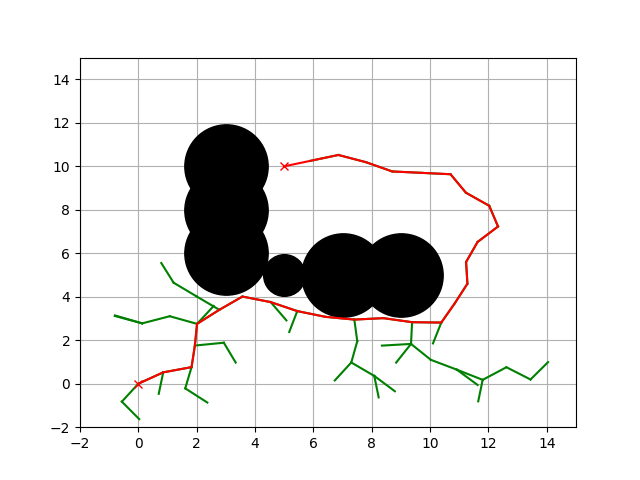
\includegraphics[scale=0.7]{Map1_1.png}
    \\Figura 1: Primera ejecución del algoritmo RRT sobre el Mapa 1.
\end{center}

\begin{center}
    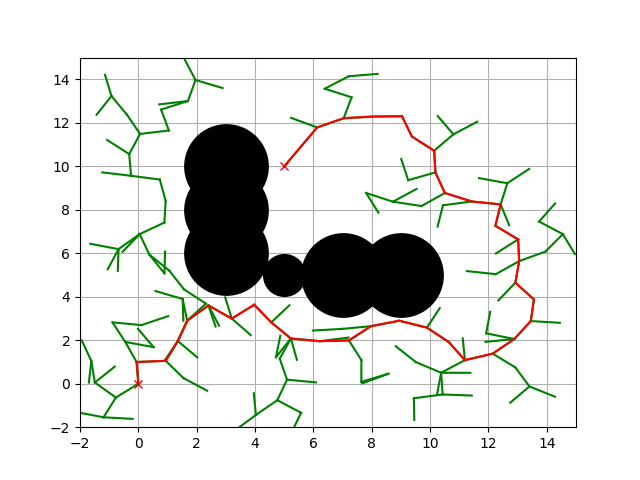
\includegraphics[scale=0.7]{Map1_2.png}
    \\Figura 2: Segunda ejecución del algoritmo RRT sobre el Mapa 1.
\end{center}

\begin{center}
    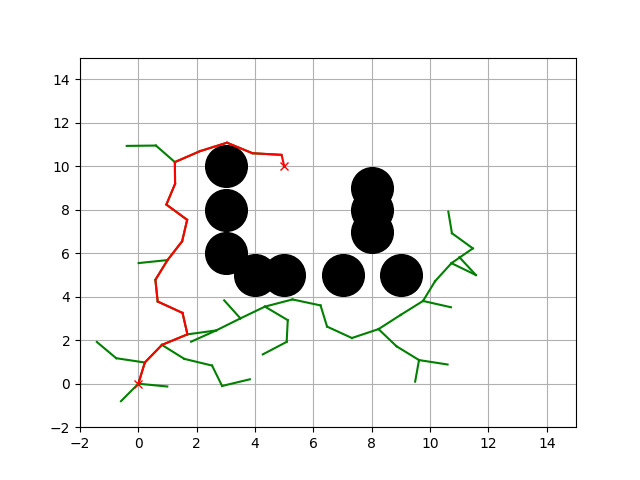
\includegraphics[scale=0.7]{Map2_1.png}
    \\Figura 3: Primera ejecución del algoritmo RRT sobre el Mapa 2.
\end{center}

\begin{center}
    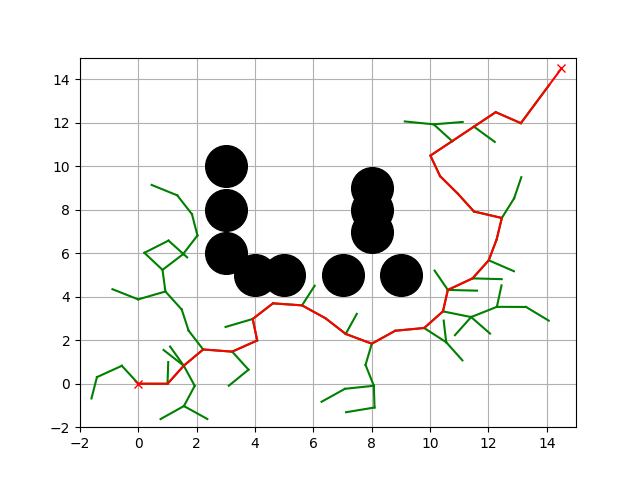
\includegraphics[scale=0.7]{Map3_1.png}
    \\Figura 4: Primera ejecución del algoritmo RRT sobre el Mapa 3.
\end{center}

\newpage
\section{Bibliografía}\label{sec:bibliografia}
\bibliographystyle{plain}
\bibliography{References}
\end{document}
